\addcontentsline{toc}{chapter}{Model danych}
Diagramy UML zwane również Unified Modeling Language umożliwiają graficzne przedstawienie logiki relacji, czy procesu \cite{diagram}. Są to standardy graficzne używane w inżynierii oprogramowania do modelowania struktury i zachowania systemów informatycznych. Umożliwiają one lepsze zrozumienie architektury systemu oraz pomagają w procesie projektowania i dokumentowania. Poniżej zostały przedstawione diagramy kolekcji występujących w bazie danych Firebase wykorzystywanych w aplikacji ZodiaCal.

\section*{Diagram bazy danych}
\addcontentsline{toc}{section}{Diagram bazy danych}

\begin{figure}[h]
	\centering
	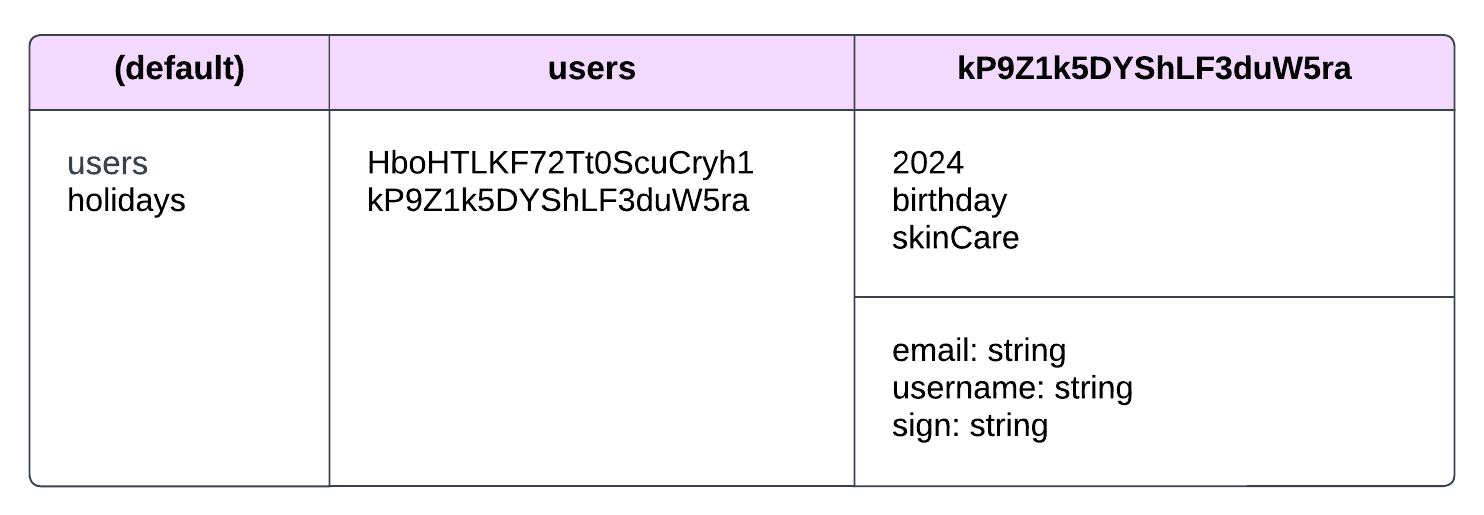
\includegraphics[width=1\linewidth]{images/model_danych/user}
	\caption{Diagram kolekcji user}
	\label{fig:user}
\end{figure}

Diagram kolekcji user (Tab. \ref{fig:user}) zawiera informację o zalogowanym użytkowniku. Każdy user posiada swój własny unikalny User UID. Podstawowe dane użytkownika to obowiązkowe pola email i user name oraz opcjonalne pole sign. Podczas korzystania z aplikacji w bazie danych tworzą się kolekcje takie jak obecny rok, w którym przechowywane są wszystkie informacje potrzebne do zarządzania kalendarzem, kolekcja birthday, w której użytkownik przechowuje daty urodzin swoich bliskich oraz kolekcję skinCare przechowujące treści dotyczące pielęgnacji cery.

\newpage

\begin{figure}[h]
	\centering
	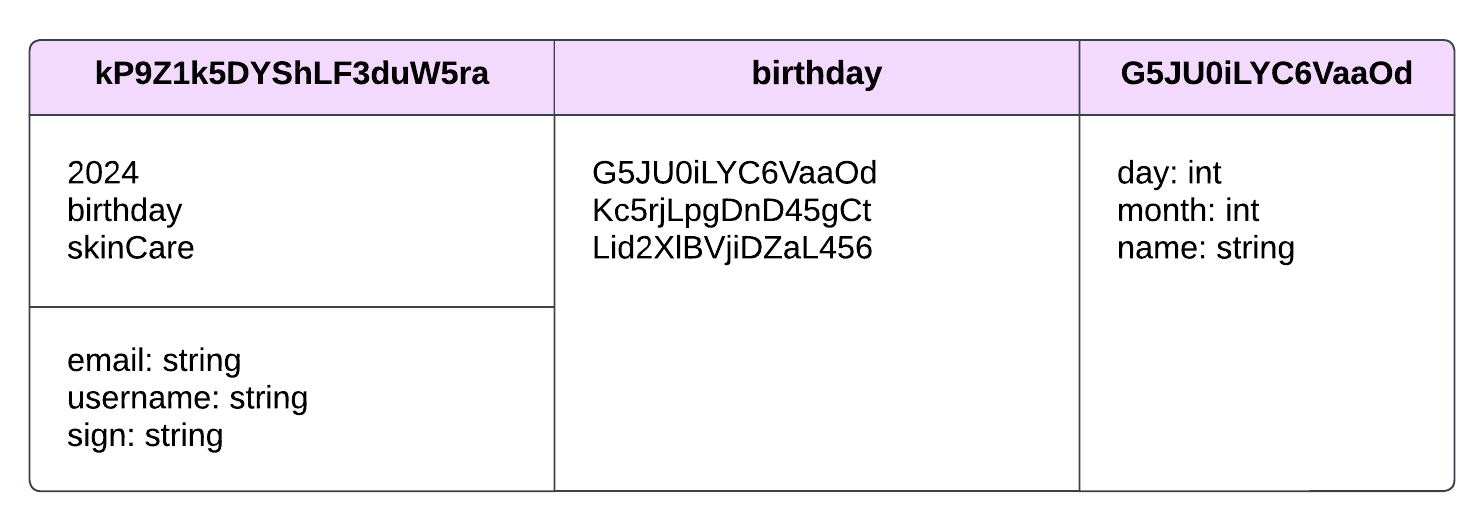
\includegraphics[width=1\linewidth]{images/model_danych/birthday}
	\caption{Diagram kolekcji birthday}
	\label{fig:birthday}
\end{figure}

Kolekcja birthday (Tab. \ref{fig:birthday}) przedstawia listę dat urodzin różnych osób. Posiada dwa pola typu int tzn. day oraz month i jedno pole typu string name, które wskazuje na imię jubilata.

\begin{figure}[h]
	\centering
	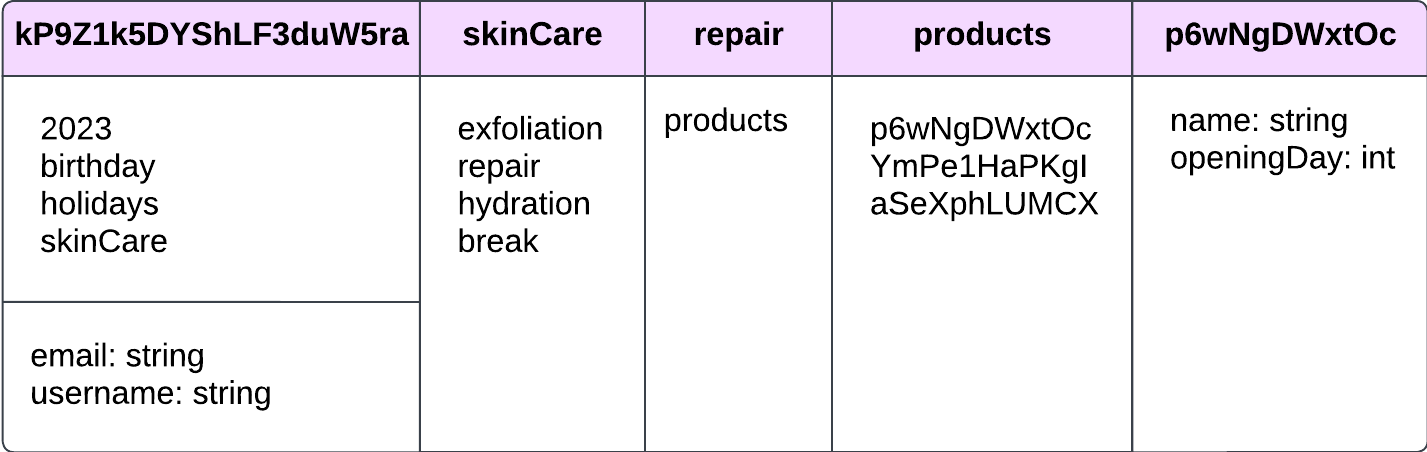
\includegraphics[width=1\linewidth]{images/model_danych/skinCare}
	\caption{Diagram kolekcji skinCare}
	\label{fig:skinCare}
\end{figure}

W tabeli o nazwie "skinCare" (Tab. \ref{fig:skinCare}), znajduje się zbiór informacji dotyczących pielęgnacji cery. W ZodiaCal zostały wyróżnione 4 rodzaje pielęgnacji: złuszczanie, odbudowa, nawilżanie oraz przerwa. Każda kolekcja danego typu pielęgnacji posiada swoje własne produkty. Produkty natomiast zawierają informację o nazwie produktu, nazwie marki oraz terminie ważności kosmetyku. Użytkownik wybiera produkty do pielęgnacji z zewnętrznego API, a następnie są one przekazywane do Firebase.

\begin{figure}[h]
	\centering
	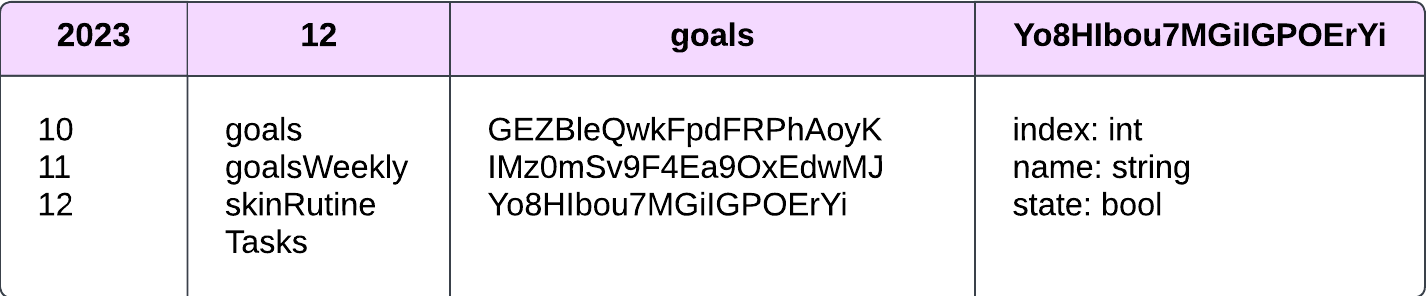
\includegraphics[width=1\linewidth]{images/model_danych/goals}
	\caption{Diagram kolekcji goals}
	\label{fig:goals}
\end{figure}

Kolekcja goals (Tab. \ref{fig:goals}) jest zagnieżdżona kolejno w kolekcji reprezentujący bieżący rok następnie bieżący miesiąc. W kolekcji odzwierciedlającej bieżący miesiąc znajdują się kolekcje dotyczące celi na dany miesiąc oraz tydzień, rutyny pielęgnacyjnej oraz zadań. Każdy cel ma swój unikalny ID, pole typu int przechowujące numer indexu, pole typu string name przedstawiające cel oraz pole typu bool state, które wskazuje czy cel został osiągnięty, czy nie.

\begin{figure}[h]
	\centering
	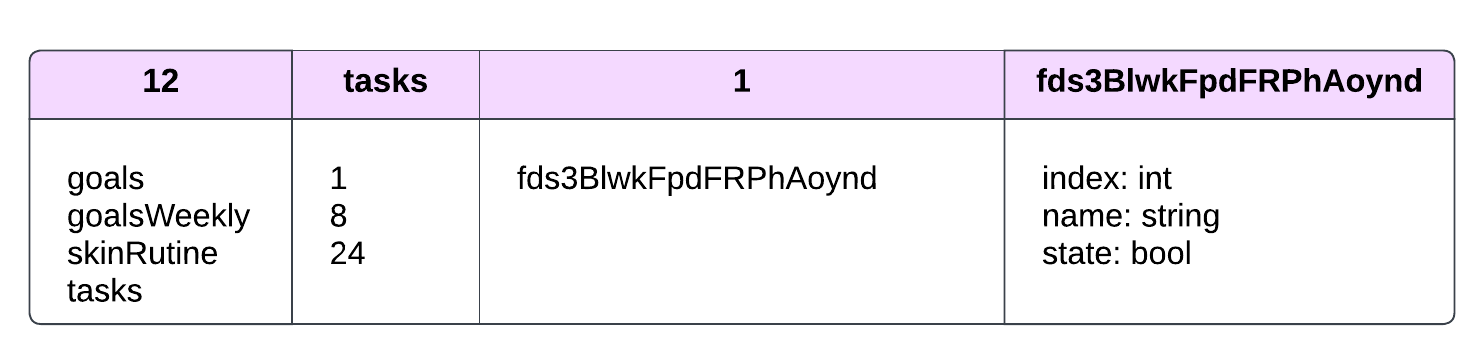
\includegraphics[width=1\linewidth]{images/model_danych/tasks}
	\caption{Diagram kolekcji tasks}
	\label{fig:tasks}
\end{figure}

Podobnie jak w przypadku kolekcji goals, tabela zatytułowana tasks (Tab. \ref{fig:tasks}) również jest zagnieżdżona w bieżącym roku oraz miesiącu. W tej kolekcji są tworzone kolejne kolekcje ilustrujące dni w danym miesiącu. Wszystkie zadania są przypisane do swoich unikalnych identyfikatorów, posiadają pola typu int, w których przechowywane są numery indeksów, pola typu string oznaczone jako "name" zawierające opis zadania, a także pola typu bool oznaczone jako "state", wskazujące na stan zadania.

\section*{Diagram UML komponentów}
\addcontentsline{toc}{section}{Diagram UML komponentów}

\begin{figure}[h]
	\centering
	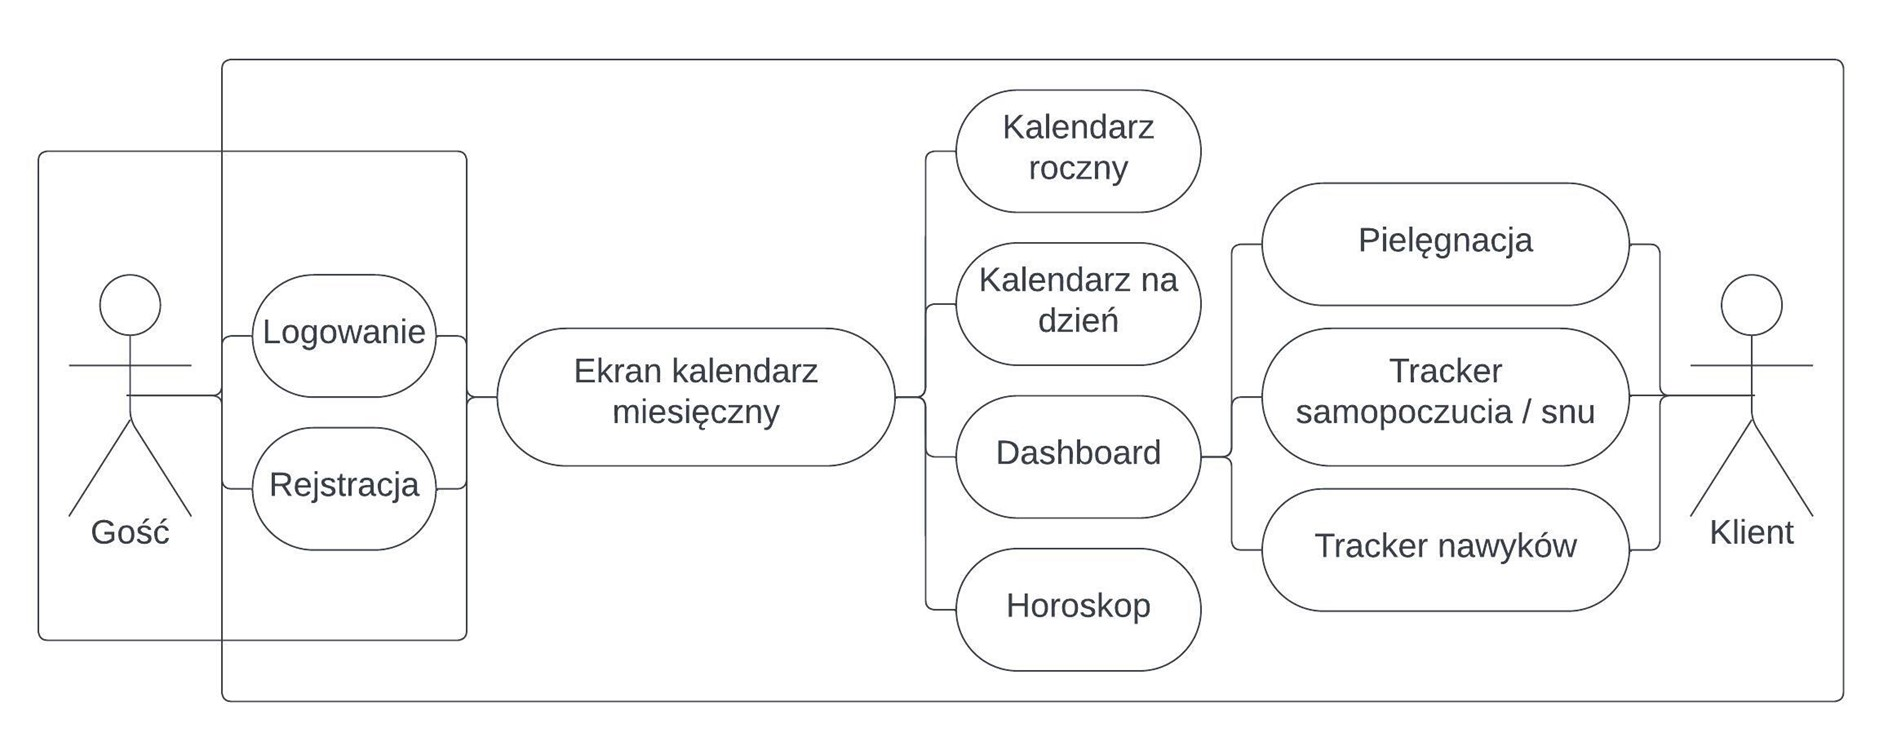
\includegraphics[width=1\linewidth]{images/model_danych/uml}
	\caption{Diagram UML komponentów}
	\label{fig:uml}
\end{figure}

NAPISAĆ CZYM SĄ KOMPONENTY!

\section*{Diagram przypadków użycia}
\addcontentsline{toc}{section}{Diagram przypadków użycia}

SKOMPRESOWAĆ ODSTĘPY + NUMERKI ZAMIAST LITER W PODLIŚCIE! + WCIĘCIE PRZYPADEK UŻYCIA

\textbf{Przypadek użycia:} Rejestracja 

\textbf{Aktor:} Gość

\textbf{Opis:} Przypadek użycia "Rejestracja" umożliwia nowym użytkownikom stworzenie konta w systemie. Rejestracja wymaga podania informacji, takich jak nazwę, adres e-mail, dzień urodzenia oraz hasło. Umożliwia to dostęp do pełnych funkcji systemu, takich jak logowanie, przeglądanie zawartości i zarządzanie swoim profilem.

\textbf{Warunki wstępne:} Gość odwiedza ekran rejestracji. Gość nie posiada konta w systemie.

\textbf{Przebieg:}

\begin{enumerate}
	\item Gość przechodzi na ekran rejestracji.
	\item System wyświetla formularz rejestracyjny.
	\item Gość wprowadza nazwę użytkownika, adres e-mail, hasło.
	\item System sprawdza poprawność wprowadzonych danych.
	\begin{enumerate}
		\item Wprowadzone dane są poprawne.
		\begin{enumerate}
			\item Użytkownik zostaj dodany do bazy danych i autmatycznie przeniesiony do ekranu głównego.
		\end{enumerate}
		\item Wprowadzone dane są niepoprawne.
		\begin{enumerate}
			\item Zostaje wyświetlony komunikat dla poszczególnych pól, że podane dane są niepoprawne. Użytkownik nie zostaje dodany do bazy danych.
		\end{enumerate}
	\end{enumerate}
\end{enumerate}


\textbf{Przypadek użycia:} Logowanie

\textbf{Aktor:} Gość

\textbf{Opis:} Przypadek użycia "Logowanie" umożliwia użytkownikom dostęp do pełnych funkcji systemu. Aby zalogować się do systemu należy podać adres e-mail i hasło.

\textbf{Warunki wstępne:} Gość uruchamia aplikację. Użytkownik niezalogowany, nieposiadający konta w serwisie.

\textbf{Przebieg:}

1. Gość uruchamia aplikację. \\
2. System wyświetla formularz logowania. \\
3. Gość wprowadza adres e-mail oraz hasło. \\
4. System sprawdza poprawność wprowadzonych danych. \\
	4.1. Wprowadzone dane są poprawne. \\
		4.1.1. Gość zostaje zalogowany do sytemu. \\
	4.2. Wprowadzon dane są niepoprawne.\\
		4.2.1. Zostaje wyświetlony komunikat, że podane dane są niepoprawne. Gość nie zostaje zalogowany do systemu.\\
		

\textbf{Przypadek użycia:} Logowanie za pomocą konta Google

\textbf{Aktor:} Gość

\textbf{Opis:} Przypadek użycia "Logowanie za pomocą konta Google" pozwala na utworzenia konta za pomocą social mediów.

\textbf{Warunki wstępne:} Gość uruchamia aplikację. Użytkownik niezalogowany, nieposiadający konta w serwisie.

\textbf{Przebieg:}

1. Gość uruchamia aplikację. \\
2. System wyświetla formularz logowania. \\
3. Gość klika w przycisk "Google".\\
4. Zostaje przeniesiony doformularza Google w którym podaje login i hasło.\\
5. Podane dane są prawidłowe. Użytkownik zostaj dodany do bazy danych i autmatycznie przeniesiony do ekranu głównego.\\


\textbf{Przypadek użycia:} Sprawdzenie horoskopu

\textbf{Aktor:} Klient

\textbf{Opis:} Przypadek użycia "Sprawdzenie horoskopu" umożliwia użytkownikom dostęp do
codziennych horoskopów dedykowany dla ich znaku zodiaku.

\textbf{Warunki wstępne:} Klient posiada konto w systemie oraz jest zalogowany. Użytkownik nie posiada przydzielonego znaku zodiaku.

\textbf{Przebieg:}

1. Klient wybiera z dolnej nawigacji zakładkę Horocop.\\
2. Zostają wyświetlone dwa, małe formularze. Użytkownik może wybrać z listy swój znak, a jeśli nie jest pewny może w drugim formularzu podać dzień i miesiąc urodzenia, a na dole zostanie wyświetlony komunikat o znaku zodiaku dla tej daty. \\
3. Znak zodiaku zostaje zapisany do bazy danych. \\
4. Po odświerzeniu strony zostaje wyświetlona nazwa znaku zodiaku, ilustracja oraz horoskop na dany dzień.\\


\textbf{Przypadek użycia:} Dodawanie urodzin do kalendarza

\textbf{Aktor:} Klient

\textbf{Opis:} W zakładce "Year" użytkownik może dodać urodziny do kalendarza, przejść do ekranu edycji listy urodzin oraz wyświetlić zaznaczone daty na kalendarzu. 

\textbf{Warunki wstępne:} Klient posiada konto w systemie oraz jest zalogowany.

\textbf{Przebieg:} 
1. Klient wybiera z dolnej nawigacji zakładkę Year.\\
2. Wprowadza w formularzu: dzień, miesiąc oraz imię solenizant.
3. System sprawdza poprawność wprowadzonych danych. \\
3.1. Wprowadzone dane są poprawne. \\
3.1.1. Urodziny zostają dodane do bazy danych oraz wyświeietlone na kalendarzu. \\
4.2. Wprowadzon dane są niepoprawne.\\
4.2.1. Zostaje wyświetlony komunikat, że podane dane są niepoprawne. Urodziny nie zostają zapisane w bazie danych. \\

\textbf{Przypadek użycia:} Edytowanie listy urodzin

\textbf{Aktor:} Klient

\textbf{Opis:} Na ekranie wyświetla się tabelą z listą urodzin użytkownika. W każdym wierszu obok imienia znajduje się ikona kosza.

\textbf{Warunki wstępne:} Klient znajduje się w zakładce "Year" oraz wyświetla mu się portal z tabelą. Dodatkowo posiada zapisane urodziny w bazie danych.

\textbf{Przebieg:} 
1. Klient wybiera z dolnej nawigacji zakładkę Year.\\
2. Klika w przycisk z ikoną ołówka, poczym zostaje wyświetlony portal.\\
3. Użytkownik klika w ikonę kosza. \\
4. Urodziny zostają usuniętę z bazy danych, a tabla zostaje automatycznie odświeżona.\\

\textbf{Przypadek użycia:} Dodawanie celów na dany miesiąc

\textbf{Aktor:} Klient

\textbf{Opis:} Na ekraniem głównym użytkownik może dodać cele na dany miesiąc.

\textbf{Warunki wstępne:} Klient posiada konto w systemie oraz jest zalogowany.

\textbf{Przebieg:} 1. Klient został pomyślnie zalogowany do systemu.\\
2. Użytkownik wpisuje w polu cel na aktualny miesiąc, a następnie klika w ikone plusa. Cel został zapisany w bazie danych.\\
3. Przycisk zmienia symbol z plusa na ołówek. Użytkownik teraz może edytować swój cel.\\
4. Gdy cel zostanie osiągnięty klient może zaznaczyć checbox, który przekreśli tekst w inpucie, a w bazie danych pole "state" zmieni swoją wartość na true.\\ 



\textbf{Przypadek użycia:} Wykreślanie zadań z listy "to do" na dany tydzień 

\textbf{Aktor:} Klient

\textbf{Opis:} W zakładce "Week" użytkownik może dodać zobaczyć listę zadań do zrobienia na dany tydzień, ma możliwośc wykreślenia zadania po jego wykonaniu. Dodatkowo może wyznaczyć cele na ten tydzień oraz dodać nowe wydarzenia oraz zadania. 

\textbf{Warunki wstępne:} Klient posiada konto w systemie, jest zalogowany oraz ma rozpisane zadania na konretne dni.

\textbf{Przebieg:} 
1. Klient wybiera z dolnej nawigacji zakładkę "Week". Na dany dzień są wpisane konkretne zadania.\\
2. Użytkownik po wykonaniu zadania klika w checbox. \\
3. Tekst w polu zostaje przekreślony, a status w bazie danych zostaje zmieniony na "true".\\


\textbf{Przypadek użycia:} Dodawanie zadań oraz wydarzeń do kalendarza dział na podobnej zasadzie jak przypadek użycia "Edytowanie listy urodzin" z tym, że tutaj w formularzu nie ma pola "Month", a w tabeli oprócz dnia, nazwy i ikony kosza jest dodatkowe pole "status" określające, czy zadanie jest ukończone.

\textbf{Przypadek użycia:} Tworzenie rutyny pielęgnacyjnej 

\textbf{Aktor:} Klient

\textbf{Opis:} Na ekranie Routines przedstawiony jest formularz dodawania produktów dla konkretnej kategorii pielęgnacji z zwenętrznej bazy danych kosmetyków.

\textbf{Warunki wstępne:} Klient znajduje się w zakładce "SkinCare" na ekranie Routines. Posiada połączenie z internetem. 

\textbf{Przebieg:} 
1. Klient wybiera z dolnej nawigacji zakładkę "SkinCare".\\
2. Z górnej nawigacji wybiera zakładkę "Routines".\\
3. Zostają wyświetlone formularze dla poszczegónych typów pielęgnacji. \\
4. Użytkownik kilka w pole "Product" i zostaje wyświetlona lista dostępnych produktów.\\
5. Użytkownik wybiera produkty z listy.\\
6. Kosmetyki zostają dodane do tabeli poniżej. \\
7. Jeśli użytkonik przez przypadek wybierze zły produkt, może go w każdej chwili usunąć z tabeli kilikając w ikone kosza.\\


\textbf{Przypadek użycia:} Monitorowanie dziennej pielęgnacji

\textbf{Aktor:} Klient

\textbf{Opis:} W zakładce "SkinCare" użytkownik może dodać zobaczyć listę kosmetyków na dany dzień w dwóch kategoriach: Morning i Evening.

\textbf{Warunki wstępne:} Klient posiada konto w systemie, jest zalogowany oraz ma ustalony plan pielęgnacji na wieczór oraz dzień.

\textbf{Przebieg:} 
1. Klient wybiera z dolnej nawigacji zakładkę "SkinCare".\\
2. W sekcji Evening użytkownik wybiera typ pielęgnacji z menu.\\
3 Zostają wyświetlone produkty dla danego typu pielęgnacji.\\
4. Użytkownik po wykonaniu pielęgnacji zaznacza klikając w chackbox, których produktów użył.\\
5. Kafelek zmienia kolor z różowego na szary.\\


\textbf{Przypadek użycia:} Podsumowanie 

\textbf{Aktor:} Klient

\textbf{Opis:} Na ekranie Summary użytkownik może zobaczyć podsumowanie swojej pielęgnacji w danym miesiącu.

\textbf{Warunki wstępne:} Klient znajduje się w zakładce "SkinCare" na ekranie Routines. W bazie danych znajdują się informację o zrealizowanych pielęgnacjach.

\textbf{Przebieg:} 
1. Klient wybiera z dolnej nawigacji zakładkę "SkinCare".\\
2. Z górnej nawigacji wybiera zakładkę "Summary".\\
3. Zostają wyświetlone wykres kołowy oraz tabela przedstawiający w ilu procentach dana pielęgnacja była w tym miesiącu złuszczająca, regenerująca, nawilżająca lub jej nie było. \\
